\documentclass[conference]{IEEEtran}
\IEEEoverridecommandlockouts
% The preceding line is only needed to identify funding in the first footnote. If that is unneeded, please comment it out.
\usepackage{cite}
\usepackage{amsmath,amssymb,amsfonts}
\usepackage{algorithmic}
\usepackage{graphicx}
\usepackage{textcomp}
\usepackage{xcolor}
\usepackage{amsmath}
\usepackage{amssymb}
\def\BibTeX{{\rm B\kern-.05em{\sc i\kern-.025em b}\kern-.08em
    T\kern-.1667em\lower.7ex\hbox{E}\kern-.125emX}}
\begin{document}

\title{IoT - Ethernet APL\\
}

\author{\IEEEauthorblockN{ Giuseppe Scalora}
\IEEEauthorblockA{\textit{Electronic Engineering} \\
\textit{Hochschule Hamm-lippstadt}\\
Lippstadt, Germany \\
giuseppe.scalora@stud.hshl.de, 10.01.2022}

}

\maketitle

\begin{abstract}
This paper will focus on the research about the communication protocol called Ethernet APL or Advanced Physical Layer. Describing how the communication occurs, what are the main characteristics and properties needed in order to make this type of communication a reality. The scope of the paper will also cover the difference between the main Ethernet protocol and the APL with a comparison with the other OSI layers used in the communication protocols. Towards the end some important main applications will be discussed and presented in order to understand the focus area of this topic alongside with the benefits and cons which this protocol can deliver.
 
\end{abstract}

\begin{IEEEkeywords}
Ethernet, communication protocols, APL, OSI layers
\end{IEEEkeywords}

\section{Introduction}
When it comes to automation networks, many challenging requirements make their appearance in the process industries. Applications of such type require continuous and stable operations working 24/7, alongside with reliability and the proper managements of thousands of signals. Then, another important factor to consider, is the usage within hazardous environments, areas in which atmosphere can be flamable or explosive, which are common in process industries. Standard Ethernet, therefore, is not considered an intrinsically safe standard for hazardous environments and a new standard had to be developed. This new standard being a newly technological Advanced Physical Layer, which will enable a much improved safety in the already existing Ethernet standard. Ethernet APL is a new standard proposed on June, 2021. As of what said, it is important to understand how new this technology is in the field.


\section{Motivation}
Nowadays process plants are seeking for an efficient engineering, fast commissioning and reliable production. The only mean to allow this is the combination of an interoperable work between industy 4.0 and the digital transformation, these allow for a higher potential which would reinforce the variables mentioned just before. The main porblems to solve being accordingly, low bandwidth, speed and/or laborious protocol conversion among the communication protocols. Therefore Ethernet APL is there to solve fill these lackings and provide an efficient digitalization on field technologies. Field devices will then be provided with enhanced connectivity, with no longer present distance and cabling problems. An insight of a possibility of having data analysis and productivity improvements is shown in Figure 1 below.\cite{b1}
\begin{figure}[htbp]
    \centerline{\includegraphics[scale=1.0]{fig1.jpg}}
    \caption{Overview on communication step through Ethernet APL \cite{b1}}
    \label{comm}
\end{figure}

 Ethernet APL as the name itself suggests, is based upon the classical ISO OSI layer, more specifically it is another one of the already known physical layers, more of this in the next sections. 

\section{State of the art}
\subsection{History of the Ethernet}
It was May 22, 1973, at Xerox Palo Alto Research Center. Bob Metcalfe started drafting the description of how an Ethernet network system, he himself invented, should work. The main principle being the interconnectivity between computing workstations and the sending of informations between computers and laser printers. This was considered as one of the best inventions at PARC, being the first high-speed LAN technology of communication. The usage of Ethernet has been a revolution in the world of technologies. Allowing for a better and improved information sharing between applications, Ethernet has become the most used internet communication protocol used throughout all the main corporations and even in domestic private use. \cite{b2}
\subsection{OSI Layer}
In order to understand what the OSI layer are and how they are defined, it is important to learn how why is it needed. The Open Systems Interconnect (OSI) model is a conceptual framework which describes communication or networking between systems, properly divided into seven layers, as to each belong an own function. The division into layers is needed to help the realisation of a communication network, with well defined levels it is made easier to find problems and understand better what is going on in a specific area of the network. The vendors in this field will always make sure to specify in which exact layer their products belong. As to the classification, it will be discussed in the following subsections.
Since the main concern of this research is to investigate and discuss in details the Physical layer or also called OSI Layer 1, the listing will start from top to bottom. The picture below will better describe and show the layers.
\begin{figure}[htbp]
    \centerline{\includegraphics[scale=0.45]{OSI-Model.png}}
    \caption{OSI layers \cite{b3}}
    \label{osi}
\end{figure}

\subsubsection{Application Layer}
Starting from layer 7, the so called application layer, is the layer which gets the closest in touch with the end-user, for example by displaying and storing information which have to be sent through a display or a communication mean. The user interacts with the software and processes of synchronisation and exchange of data but it does not touch directly the application itself. Examples of this include Web Browsers such as Firefox or Chrome, which display web pages through HTTP communication, or TelNet. 
\subsubsection{Presentation Layer}
The presentation layer or layer 6 is where encapsulation, encryption and decryption of data happen. It creates a communication bridge between network and application via proper translation of data. Also called syntax layer because it makes sure that an independence between data representation and data translation is present. Example of this is the conversion from and to a data structure file of XML type.
\subsubsection{Session Layer}
The layer 5, as the name suggests already, creates and handles a session between two or more computers. It provides the capability of checkpointing, recovery, resuming and terminating a session, functions commonly used in internet protocols such as TCP. Its implementation is performed mostly by using remote procedure calls which allow the programmer to execute processes on a remote machine, triggered by the machine being in used.
\subsubsection{Transport Layer}
The transport layer manages the exchange and transmission of data sequences  with variable lengths between a source and a destination host. It thoroughly controls over the transmission making sure that the processes of segmentation and desegmentation occur properly. If some data has not been delivered correctly, it is the job of the transport layer to make sure that that portion of data gets recovered and then redelivered correctly. In our everyday´s life we can see the transport layer being applied to the UDP or TCP internet ports, entities which can allow or not allow the transmission of data through them. 
\subsubsection{Network Layer}
If the transport layer deals then with ports in UDP and TCP protocols, the network layer handles the IP addresses of a network. It pratically deals with the main router functionalities and communication between routers. If there is an ingoing or outgoing connection from a router to a server, the first has to make sure that the sending and receiving of packets gets executed and routed using the most feasible and efficient track/route among the millions available in the distributed system.
\subsubsection{Data Link}
The layer 2, processes the transmission and node to node communication. Working on top of the physical layer, can detect and correct errors which can occur in the latter. The data link layer is a bit of an exception compared to the others, as it possesses two sublayers the MAC or Media Access Control and the LLC, logical link control. 
The MAC is responsible to allow the access to the media, working in form of centralized or distributed control. Both handling the communication between nodes. The MAC specifically handles the frame synchronization which is responsible to determind the start and end of a bitstream transmission. 
The LLC, on the other hand, multiplexes the running protocols of the data link layer and determines the mechanisms used for addressing and controlling the communication exchange between sending and recipient machine.
\subsubsection{Physical Layer}
The physical layer is where the electrical conversion happens. The streams of raw data gets converted from digital to electrical or radio signals. Within the specifications of the layer, voltage levels, impedances, pin layouts, frequency, cable construction parameters and timing are almost always present. Technically the physical layer is nonetheless the physical representation of the system. Bluetooth, Ethernet and USB are standards examples of the Physical layer.
\cite{b4}\cite{b5}
\section{Ethernet Advanced physical layer}
Ethernet APL is considered to be a subset of the common standardized communication protocol, Ethernet. Ethernet-APL brings all the standardized Ethernet technology to the table, alongside with all its advantages and even more. This results in being very helpful in the application for process plants or industrial processes. As Ethernet APL makes sure that long distance communication occurs in the most qualitative possible way. Working alongside major organizations, the process industries were brought to the point of specifying one single physical layer which could also be applied and satisfies the requirements of process automation together with providing connectivity with broadly distributed, two-wire, loop-powered field instruments in potentially hazardous environments. APL reached a significant achievement which comes with an increased available bandwidth for digital communication, simplifying the typical network architecture. Based on Ethernet, as already mentioned, APL improves and facilitates cybersecurity and it also eliminates the need of converting the communication protocol from field device to business systems or to the cloud, wrapping the communication in an all-in-one protocol. Therefore as an introduction for the Ethernet APL, we can obviously state that, as a subset of the traditional Ethernet, its main area of focus is process automation, IoT communication protocols, control systems and safety in hazardous areas.
\begin{figure}[htbp]
    \centerline{\includegraphics[scale=0.45]{Field-commAPL.png}}
    \caption{Overview of field communication using APL \cite{b6}}
    \label{fca}
\end{figure}
\subsection{Standards of APL}
IEEE recently approved a new standard called 802.3cg-2019 or 10BASE-T1L, which basically extends the normal Ethernet standard 802.3 up to the inclusion of wiring a single pair over a long distance of up to 1000, which can also allow supplying power to the field devices. Now according to these technical standards and in order to approve the concept of APL and its usage in process plants, some extended standards need to be defined. Thus, with the advent of APL now the 10BASE-T1L standard has been extended furthermore especially for usage in hazardous areas.
Ethernet APL standards will define port profiles for various power levels, in order to be used in and outside hazardous areas. This makes sure that the interoperability of APL switches and devices is not compromised and that power delivery will replace the optional power data line already within the 10BASE-T1L standard.
APL will deliver power to the devices much safer intrinsically compared to other famous communication protocols such as Profibus or HART. As supported by the executive vice president of Pepperl+Fuchs, Michael Kessler, this leads in a change of wiring construction which will now allow for the design of two wired instruments instead of the traditional four wires, due to high power.
Another important standardization concerns the field of ASIC, application specific integrated circuits. Before the APL can enter the market as a commercializable option, ASIC need to be able to support APL and all its characteristics. \cite{b6}


\subsection{Main characteristics}
To dive in deeper into the specifics. Ethernet APL makes use of a two-wired instrinsically safe technology. Now, taking a look at Fig.3, we can see how a field installation of APL looks like, having two separate big segments called zones and divisions. With a structure based upon trunk and spur installations let us take a look at the difference between the two of them. Two segments include accordingly trunk and spur lines. Trunk lines deliver power to the field switches for up to 1000 meters while spur lines deliver signals up to 200 meters to the field devices or instruments. At the end of each trunk line there are APL field switches which provide for up to 60 Watts of power and multiple connections with up to 50 devices, on the other hand, anchored to the spur lines are the part of the switches which the communication signals to all the devices. An example of how the trunk/spur wiring looks like, is shown below.
\begin{figure}[htbp]
    \centerline{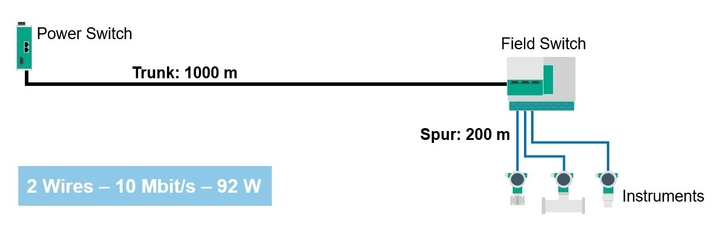
\includegraphics[width=90mm, height=40mm, scale=0.5]{trunkspur.jpg}}
    \caption{Trunk and spur wired connection example \cite{b7}}
    \label{trsp}
\end{figure}

Specifically for Ethernet APL there are two types of switches. The field switch, which receives power from the trunk lines in zone 1/Div. 2 and which holds the following characteristics (For a better understanding please take a look at the zones/divisions in Fig.3):
\begin{enumerate}
\item Intrinsically safe outputs for spur lines.
\item Instruments in Zone 0/Div. 1.
\item Field installations in Zone 1/Div. 2.
\end{enumerate}

Other than field switches, guided DIN switches are also present within an APL installation. These instead connect the spur lines to the Ethernet installation. They hold the following specfics:
\begin{enumerate}
\item Power supply and communication over spur lines.
\item Installations in Zone 2/Div. 2.
\item Outer powering from outer source.
\item Redundancy support on Ethernet plant level.
\end{enumerate}

In a typical APL installation there is also a third switch called power switch, as the word already suggests, this switch is present at the beginning of the trunk line and makes sure to supply power to the trunk line from a control station and it is directly connected to the Ethernet APL network.
Moving on in terms of communication, Ethernet APL provides for up to 10 Mbps, in full duplex mode, through lines of up to 1000 meters long which makes it one of the most efficient and fastest ways of communications for long distances on a two wired pair of cables and for a switched type of network.
The characteristics of a typical APL network, render the field perfect for scalability in terms of devices and switches connected to the network. Since the ethernet APL is suitable for transportation of higher level layers functions it holds some particularly useful related characteristics, such as automatic detection of neighborhood switches which helps the device exchanges, parallel multiple connections communicating at the same time and fully operable by the user without compromising the efficiency and last but not least possessing ring redundancy and resilience makes sure that the communications are automatically re-routed in case of faults or interruptions at trunk or spur level.
The last important factor which is to be taken into consideration when talking about APL`s main characteristics is the type of connections and connectors used. Starting with the cables, the ones used in an APL network are compliant with the standard IEC 61158-2, Type A, 100 Ohm resistance and intrinsically safe, which are also the already used standard ones for fieldbus. Also the standard IEC TS 60079-47 (2-Wire Intrinsically Safe Ethernet) provides a high protection and safety against explosions and hazards. The connections between wires are polarity independent, which helps avoiding errors during installations and the physical connections occur in a very simplistic way using only Spring-clamp type of terminals, screw type and M8 and M12 connectors. Typical APL cables and connectors would look like the following.\cite{b8}
\begin{figure}[htbp]
    \centerline{\includegraphics[scale=0.20]{connectors.png}}
    \caption{Connectors for APL network \cite{b9}}
    \label{conn}
\end{figure}
The standards used for the connection types deliver a simple and fast way of migrating the installation to a different type of communication if it would be needed to.
\subsection{Ethernet APL against the world}
To understand the advantages of the adoption of APL against the competitors, a small table is shown below with the main characteristics among 4 different types of protocols.
\begin{figure}[htbp]
    \centerline{\includegraphics[scale=0.40]{table.png}}
    \caption{Comparison table between protocols \cite{b8}}
    \label{table}
\end{figure}
Now, let us analyze the table. APL results to be the fastest in terms of communication through long distances and the most feasible one for instrinsically safe scenarios with the possession of construction technologies equal to the fieldbus technology but with the advantage of having single network technology from field to enterprise and an always present polarity independence.
\section{APL application challenges}
Some challenges of APL application appear when it comes to field devices protections. The ability to write on a device should be selectable via means of software or hardware and routine tests should allow the deactivation of the writing protections. This still looks like an ideal solution to which a solution has to be given. Next up on the list regards the field devices having to be unified for the current standards of the plant. Since plants have a longer lifetime compared to field devices, these last ones have to comply to the plants standard even when being updated and improved without causing faults or disrupting functionalities. In short, compatibility problems have to be fixed in order to have a fully unified installation. Lastly, the costs of an APL installation with its advanced technologies must justify for the use of at least 80\% of APL devices in the installation to not render the costs too expensive proportioned to its realization.\cite{b10}
\section{Main application and importance in process plants}
An important statement comes from the technological leader Pepperl-Fuchs. According to this technological giant, industry 4.0 and IIoT have been longly part of daily life. Although in smart factories it has been a problem because of the lack of high speed end to end data transmission. This lack is of course filled by the advent of APL Ethernet. According to this, Pepperl-Fuchs suggests that in the near future an extensive use of APL will be applied to process plants.
Let us now take a look at this main application of the Ethernet APL for IoT purposes and industrial purposes.
The main application of Ethernet APL in a plant is touching one of the most important plant related topics, which is efficiency. For a plant to be efficient, it must be reliable, able to inform and provide data for future maintenance of tools and instrumentation, must be easy to diagnose if any accident happens and needs to be flexible to work with different devices manufacturers. Continuous collection of data in real time makes sure that APL supports all the mentioned requirements of a plant. Let us see how APL does that in a real world application:
\begin{itemize}
\item APL provides reliability as a well proven ethernet standard as it has been a standard for many years in the IT world, useful for hybrid and process automation.
\item APL is highly available as the protocol features availability concepts like system redundancy or media redundancy for cable accidents.
\item Predictive maintenance provided by the APL protocol includes all the smart field devices which make sure the communication renders the data accessible and available for status monitoring and condition monitoring.
\item Ethernet technology provides for easy network diagnostic tools to identify causes of failures and accidents and keep track of the current status of any switch or front/end device in the system.
\item Lastly, but not in importance, the interoperability provided by APL ensures the correct working functionalities of devices from different manufacturers and vendors.
\end{itemize}
The access to field data activates new digital services needed by the business management of the process plant. By an extensive inclusion of IIoT technology it provides real time feedbacks and information.


\section{Conclusion}
The idea of having an ethernet with an advanced physical layer is indeed a great step towards an internet communication protocol which could bring and lead to amazing improvements in the field. With its main characteristics compared to other protocols it is clear that as soon as it will become a more standardized communication mean, it will overtake even its competitors. Now the paper has given a broad enough overview and bit of information necessary as an input for further research of the topic. Leaders of technological corporations are collaborating in order to finalize the process of delivery for the APL and we might see even a broader range of applications very soon as shown in the delivery roadmap below for the APL.
\begin{figure}[htbp]
    \centerline{\includegraphics[scale=0.45]{apllaunchroadmap.png}}
    \caption{Roadmap for development of APL \cite{b8}}
    \label{rmapl}
\end{figure}



\begin{thebibliography}{00}
\bibitem{b1} https://www.analog.com/en/thought-leadership/ethernet-apl-optimization-of-process-automation.html
\bibitem{b2} C. Spurgeon, Ethernet. Beijing: O'Reilly, 2009.
\bibitem{b3} https://www.educba.com/what-is-osi-model/
\bibitem{b4} https://www.networkworld.com/article/3239677/the-osi-model-explained-and-how-to-easily-remember-its-7-layers.html
\bibitem{b5} https://en.wikipedia.org/wiki/OSI\_model
\bibitem{b6} https://www.controlglobal.com/articles/2020/advanced-physical-layer-standard-to-make-field-level-ethernet-a-reality/
\bibitem{b7} https://www.pepperl-fuchs.com/italy/it/41850.htm
\bibitem{b8} https://www.ethernet-apl.org/
\bibitem{b9} https://www.automationworld.com/communication/article/21545085/industrial-ethernet-advances-broaden-the-networks-value-across-industries
\bibitem{b10} Whitepaper Ethernet-APL in the Field for
high-availability Safety Applications
\end{thebibliography}

\end{document}
